\vspace{-0.1cm}
\section{Background and Related Work}
\label{sec:background}

We first introduce %formal 
notations useful for the rest of the paper (Section~\ref{sec:notation}). Then, we review %in detail previously proposed 
existing time-series anomaly detection methods (Section~\ref{sec:ad_methods}), and discuss their limitations when applied to large heterogeneous sets of time series (Section~\ref{sec:limitation}). 


\vspace{-0.2cm}
\subsection{Time-Series and Anomaly Score Notations}
\label{sec:notation}

%In this section, we review notations for time series and anomaly score sequences.

\textbf{Time Series: }A time series $T \in \mathbb{R}^n $ is a sequence of real-valued numbers $T_i\in\mathbb{R}$ $[T_1,T_2,...,T_n]$, where $n=|T|$ is the length of $T$, and $T_i$ is the $i^{th}$ point of $T$. We are typically interested in local regions of the time series, known as subsequences. A subsequence $T_{i,\ell} \in \mathbb{R}^\ell$ of a time series $T$ is a continuous subset of the values of $T$ of length $\ell$ starting at position $i$. Formally, $T_{i,\ell} = [T_i, T_{i+1},...,T_{i+\ell-1}]$. %We then define 
A dataset $\mathcal{D}$ is a set of time series. 
Note that the time series contained in $\mathcal{D}$ can be of diverse lengths. We define the size of $\mathcal{D}$ as $|\mathcal{D}|$.

\textbf{Anomaly Score Sequence: }For a time series $T \in \mathbb{R}^n $, an anomaly detection method (or detector) $D$ returns an anomaly score sequence $S_T$. For point-based approaches (i.e., methods that return a score for each point), we have $S_T \in \mathbb{R}^n$. For subsequence-based approaches (i.e., methods that return a score for each subsequence of a given length $\ell$), we have $S_T \in \mathbb{R}^{n-\ell}$ and $S_T = [{S_T}_1,{S_T}_2,...,{S_T}_{n-\ell}]$ with ${S_T}_i \in [0,1]$. In most applications, the anomaly score has to be the same length as the time series. Thus, for subsequence-based approaches, we define $S_T = [{S_T}_1]_{i\in[0,\ell/2]} + [{S_T}_1,{S_T}_2,...,{S_T}_{n-\ell}] + [{S_T}_{n-\ell}]_{i\in[0,\ell/2]}$ with $|S_T| = |T|$.

\textbf{Anomaly Detection Accuracy: }For a time series $T \in \mathbb{R}^n $, an anomaly detection method (or detector) $D$ that returns an anomaly score sequence $D(T) = S_T$ and labels $L \in [0,1]^n$ that indicated with 0 or 1 if the points in $T$ are normal or abnormal respectively, we define $Acc:\mathbb{R}^n,\{0,1\}^n \rightarrow [0,1]$ as an accuracy function for which $Acc(D(T),L)$ indicates how $D$ is accurate (i.e., and produce an anomaly score close to 1 when the label is equal to 1) when applied on $T$ and accordingly to $L$. The closer to one, the better.

\begin{figure}
    \centering
    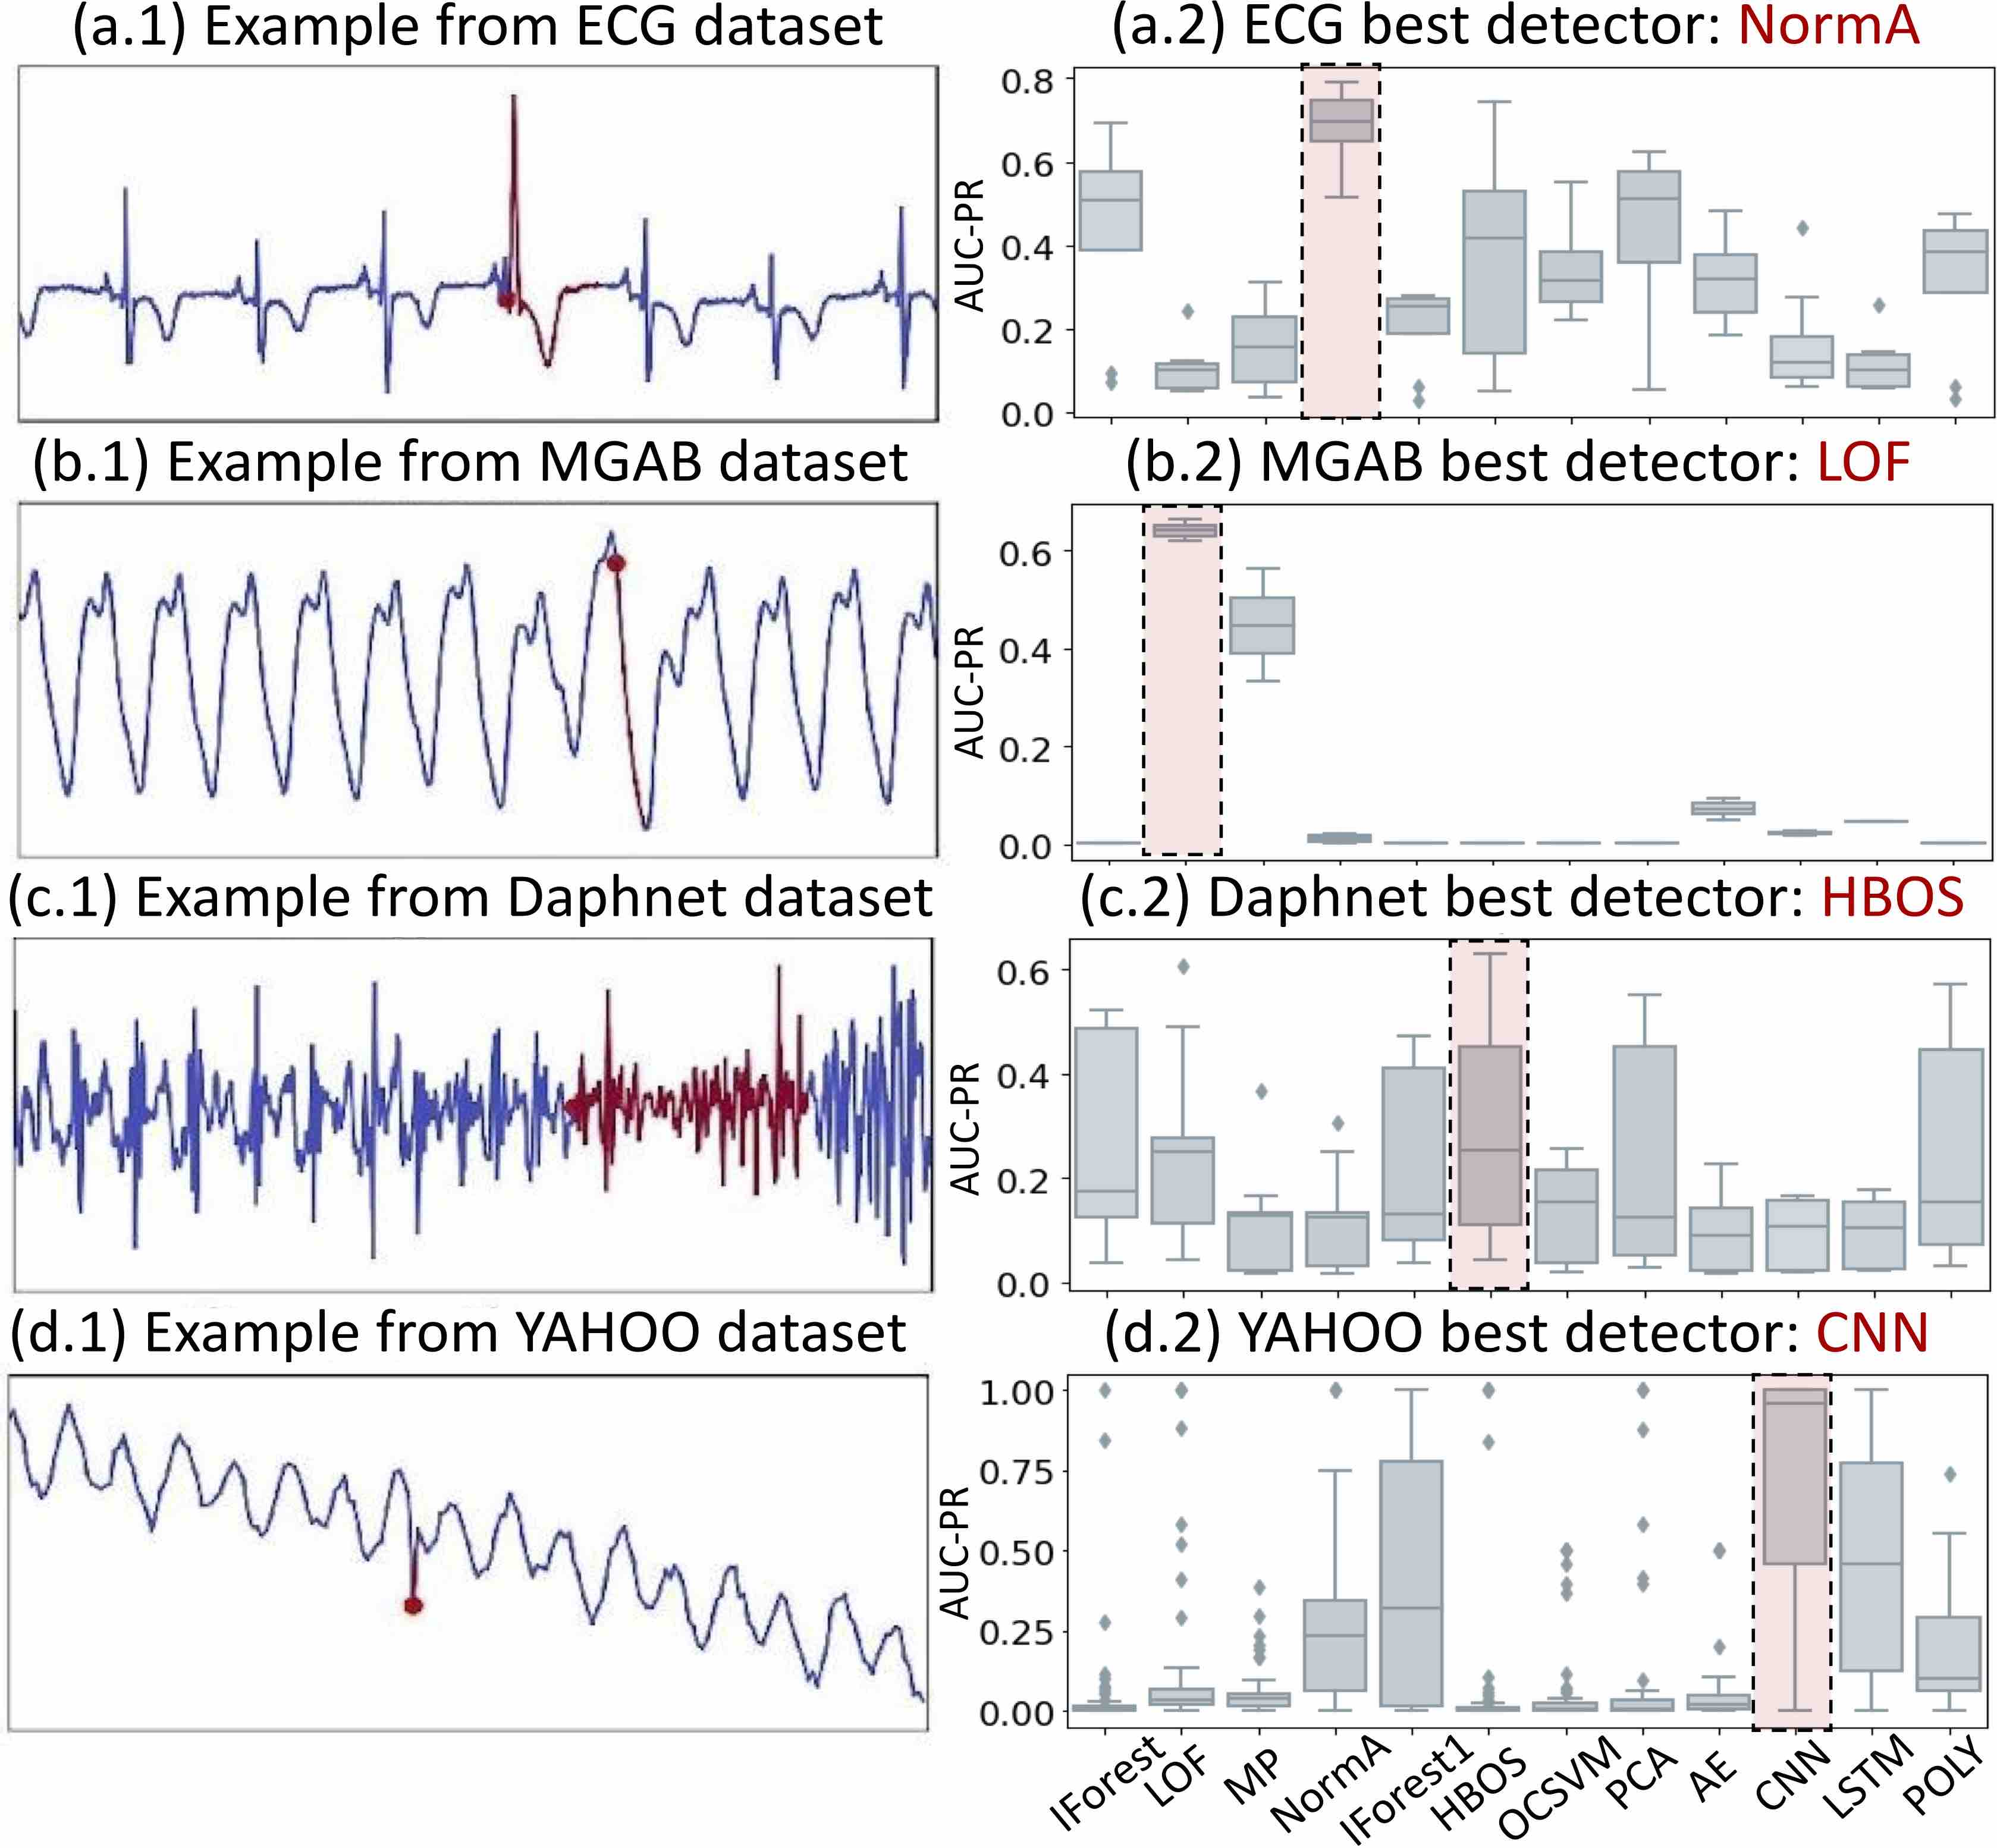
\includegraphics[width=0.91\linewidth]{figures/2_diversity_method.jpg}
    \vspace{-0.3cm}
    \caption{Accuracy of 12 anomaly detection methods on 4 datasets.}
    \vspace{-0.3cm}
    \label{fig:diversity}
\end{figure}

\vspace{-0.2cm}
\subsection{Anomaly Detection Methods for Time Series}
\label{sec:ad_methods}

%Anomaly detection in time series is a crucial task for many relevant applications. %Therefore, 
Several different methods (for diverse types of time series, or applications) have been proposed in the literature. One type of anomaly detection method is \textit{discord-based methods}. These methods focus on the analysis of subsequences for the purpose of detecting anomalies in time series, mainly by utilizing nearest neighbor distances among subsequences \cite{DBLP:conf/icdm/YehZUBDDSMK16,DBLP:conf/edbt/Senin0WOGBCF15,Keogh2007,Liu2009,DBLP:conf/adma/FuLKL06,DBLP:conf/sdm/BuLFKPM07,DBLP:journals/datamine/LinardiZPK20}. 

Instead of measuring nearest neighbor distances, \textit{proximity-based methods} focus on estimating the density of particular types of subsequences in order to either extract a normal behavior or isolate anomalies. As a subsequence can be seen as a \syl{multidimensional} point (with the number of dimensions corresponding to the subsequence length), general outlier detection methods can be applied for time series anomaly detection~\cite{liu_isolation_2008,Breunig:2000:LID:342009.335388,ma2020isolation}. Among them, Isolation Forest~\cite{liu_isolation_2008} has been shown to work particularly well for time series anomaly detection task~\cite{Series2GraphPaper}. Moreover, recent proximity-based methods dedicated to identifying abnormal subsequences in time series have been proposed. For instance, NormA, a proximity-based method that first clusters data to obtain the normal behavior~\cite{norm, boniol_unsupervised_2021, DBLP:conf/icde/BoniolLRP20, boniol2021sand, boniol2021sanddemo}, %or Series2Graph that converts the time series into a graph to facilitate the detection of anomalies~\cite{Series2GraphPaper}, 
has been shown to achieve strong performance.

Furthermore, \textit{forecasting-based methods}, such as recurrent neural network-based ~\cite{malhotra_long_2015} or convolutional network-based ~\cite{8581424}, have been proposed for this task. Such methods use the past values as input, predict the following one, and use the forecasting error as an anomaly score. Such methods are usually trained on time series without anomalies, or make the assumption that the anomalies are significantly less frequent than the normal behaviors.

Finally, \textit{reconstruction-based methods}, such as \syl{autoencoder} approaches ~\cite{10.1145/2689746.2689747}, are trained to reconstruct the time series and use the reconstruction error as an anomaly score. As both forecasting and reconstruction-based categories detect anomalies using prediction errors (either forecasting or reconstruction error), we can group them into \textit{prediction-based methods}. 

\vspace{-0.2cm}
\subsection{Limitations of Anomaly Detection Methods} % on heterogeneous data}
\label{sec:limitation}

Recent benchmarks and experimental evaluations have been proposed in the literature~\cite{10.14778/3538598.3538602, 10.14778/3551793.3551830, kdd21}. Such benchmarks provide a large collection of time series from various domains and evaluate multiple methods belonging to the categories mentioned above. However, these experimental evaluations led to the same conclusion: no method exists that outperforms all the others on all time series from various domains. Figure~\ref{fig:diversity}, which depicts the accuracy of 12 diverse anomaly detection methods\footnote{We use 12 methods that have been employed in previous studies ~\cite{10.14778/3529337.3529354, 10.14778/3551793.3551830}. Note that other methods and variations exist that may lead to improved results.} on four time series datasets, illustrates the conclusion above. In Figure~\ref{fig:diversity} (a.2), we observe that NormA is the most accurate model on the ECG dataset~\cite{Moody} (a time series example is depicted in Figure~\ref{fig:diversity} (a.1)). However, Local Outlier Factor (LOF)~\cite{Breunig:2000:LID:342009.335388}, and Matrix profile (MP)~\cite{DBLP:conf/icdm/YehZUBDDSMK16} are significantly outperforming NormA on the MGAB dataset~\cite{markus_thill_2020_3762385} (see Figure~\ref{fig:diversity} (b.2)), whereas CNN~\cite{8581424} is outperforming NormA, LOF, and MP on the YAHOO dataset~\cite{yahoo} (see Figure~\ref{fig:diversity} (d.2)). The following two reasons explain this large difference in performance among datasets.

\vspace{-0.1cm}
\subsubsection{\textbf{Heterogeneity in anomaly types}}

First, There are three types of time-series anomalies: \textit{point}, \textit{contextual}, and \textit{collective} anomalies. \textit{Point} anomalies refer to data points that deviate remarkably from the rest of the data. Similarly, \textit{Contextual} anomalies refer to data points within the expected range of the distribution (in contrast to point anomalies) but deviate from the expected data distribution, given a specific context (e.g., a window). For instance, Figure~\ref{fig:diversity} (d.1) illustrates a time series from the YAHOO dataset with a \textit{Contextual} anomaly. The value of the anomalies is inside the range of normal values\syl{, but} is abnormal in the context of the distribution of values of the surrounding point. For this particular types of anomalies, \textit{reconstruction} and \textit{forcasting}-based methods are particularly accurate (as shown in Figure~\ref{fig:diversity} (d.2))

\textit{Collective} anomalies refer to sequences of points that do not repeat a typical (previously observed) pattern. The first two categories, namely, point and contextual anomalies, are referred to as \textit{point-based} anomalies, whereas \textit{collective} anomalies are referred to as \textit{subsequence} anomalies. For instance, Figure~\ref{fig:diversity} (a.1), (b.1), and (c.1) show three time series with sequence anomalies. However, even for time series belonging to the same anomaly type categories, we observe that the most accurate models are all different.  

\vspace{-0.1cm}
\subsubsection{\textbf{Heterogeneity in time series structures}}

This diversity in model accuracy can be explained by other factors related to the time series structures. Indeed, on top of these categories mentioned above, the combination of them also matters. First, we need to differentiate time series containing \textit{single} anomalies from time series containing \textit{multiple} anomalies. Last, the \textit{multiple} time series category has to be divided into two subcategories, namely time series containing \textit{multiple different} and \textit{multiple similar} anomalies. For instance, methods based on neighbor distance computation such as LOF are very accurate in detecting \textit{single} or \textit{multiple different} anomalies, but less accurate for \textit{multiple similar}. To illustrate this point, Figure~\ref{fig:diversity} (a.2) depicts the results of 12 anomaly detection methods on the ECG dataset (that contains \syl{}%a large number of 
\textit{multiple similar} anomalies), for which LOF accuracy is low. On the contrary, Figure~\ref{fig:diversity} (b.2) depicts the results of the same 12 anomaly detection methods on the MGAB dataset (that contains \syl{}%few
\textit{multiple different} anomalies), for which LOF accuracy is high.

On top of the large variety of time series and anomaly characteristics mentioned above, time series can have distinct statistical characteristics, resulting in an even larger variability in the accuracy of anomaly detection methods. %To all these differences between time series, resulting in large variability in the accuracy of anomaly detection methods, we can add differences in the time series statistical characteristics. 
The latter can be the differences between \textit{stationary} (i.e., with a constant distribution of values over time) and \textit{non-stationary} (i.e., with a changing distribution of values over time) time series, or \textit{single normality} (i.e., time series containing only one normal behavior) and \textit{multiple normalities} (i.e., time series containing multiple normal behaviors) time series. 

\vspace{-0.1cm}
\section{Motivation and Problem}
\label{sec:problem_def}

In this section, we describe solutions that can be applied to solve the limitations mentioned above, and we motivate the benefits of these solutions. We finally formally define the problem.

\vspace{-0.1cm}
\subsection{Ensembling Detectors}

% The first solution is to ensemble the anomaly scores produced by all the detectors. Multiple ensembling techniques have been proposed in the literature~\cite{10.1145/2830544.2830549} from which two main methods arise: (i) \textit{Averaging}: the average of the anomaly scores for each timestamp, (ii) \textit{Maximizing}: the maximum anomaly score for each timestamp (iii) \textit{Average of Maximum}: the average of the maximum for \syl{a randomly selected subset} of detectors. \textit{Averaging} strategy is proven to be the more robust and low-risk strategy compared to the other two~\cite{10.1145/2830544.2830549}. Formally, for a given time series $T$ of length $n$ and a set of detectors $\mathcal{B}$, \textit{Averaging} strategy is defined as  $Avg.Ens.=[Avg_1,Avg_2, ..., Avg_m]$ with $Avg_i$ (for $i \in [i,m]$) equals to:
% %\[
% $Avg_i= (1/|\mathcal{B}|)\sum_{D \in \mathcal{B}} D(T)_i$.
% %\]

The first solution is to ensemble the anomaly scores produced by all the detectors. Multiple ensembling techniques have been proposed in the literature~\cite{10.1145/2830544.2830549} from which two main methods arise: (i) \textit{Averaging}: the average of the anomaly scores for each timestamp, (ii) \textit{Maximizing}: the maximum anomaly score for each timestamp (iii) \textit{Average of Maximum}: the average of the maximum for \syl{a randomly selected subset} of detectors. \textit{Averaging} strategy is proven to be the more robust and low-risk strategy compared to the other two~\cite{10.1145/2830544.2830549}. \syl{Formally, the \textit{Averaging} strategy is defined as follows:

\vspace{-0.1cm}
\begin{definition}
    Given time series $T$ of length $n$ and a set of detectors $\mathcal{B}$, \textit{Averaging} strategy is defined as $Avg~Ens = [Avg_1,Avg_2, ..., Avg_m]$ with $Avg_i$ (for $i \in [i,m]$) equals to $Avg_i= (1/|\mathcal{B}|)\sum_{D \in \mathcal{B}} D(T)_i$.
\end{definition}
}
\vspace{-0.1cm}

In the rest of the paper, we call the \textit{Averaging} strategy \textit{Averaging Ensemble (Avg Ens)}. As depicted in Figure~\ref{fig:intro_fig} (a), which shows the accuracy of detectors (in grey) and the Averaging Ensemble (in orange), we observe that such a strategy already outperforms all existing approaches. Nonetheless, such a method requires running all detectors to produce one ensembled anomaly score, resulting in a costly execution time (see Figure~\ref{fig:intro_fig} (b)). In a scenario with very long time series and an increasing number of detectors to consider, such an approach is not sustainable and feasible in practice.

\vspace{-0.1cm}
\subsection{Model Selection}

A solution to tackle the limitations mentioned above is to apply model selection based on the characteristics of the time series. The main idea is to train a model to automatically select the best detector (anomaly detection method) for a given time series. In such a case, the user only has to run one model, drastically limiting the execution time required. This topic has been tackled in several recent papers related to AutoML (Automatic Machine Learning). Recent approaches, such as MetaOD~\cite{NEURIPS2021_23c89427, https://doi.org/10.48550/arxiv.2009.04395}, explored meta-learning to identify the best outlier detection algorithm on tabular datasets. 
%Recent studies have also been proposed for the specific case of time series~\cite{https://doi.org/10.48550/arxiv.2009.04395, https://doi.org/10.48550/arxiv.2102.05740}. 
These research works rely on pre-computed models' performances on a subset of datasets to learn a mapping from the dataset's characteristics to the detectors' performance. Methods have been proposed to select models in an unsupervised way~\cite{https://doi.org/10.48550/arxiv.2210.01078}, but require running multiple models in advance, which (like Averaging Ensemble) limit the applicability due to high cost.
%Overall, existing AutoML solutions require (i) a universal objective function among models, which is not applicable to anomaly detection methods; (ii) a predefined set of features, which is difficult to obtain for time series due to varying lengths and the lack of standardized featurization solutions; (iii) running multiple anomaly detection methods several times, which is prohibitively expensive in practice. 

\vspace{-0.1cm}
\subsection{Classification for Model Selection}

In general, for the specific case of time series, most of the work described above and future AutoML methods will rely on time series classification methods for the model selection step. In such a case, the method aims to classify time series into classes corresponding to the available anomaly detection methods. One time series must be classified into the detector class that maximizes anomaly detection accuracy. However, no existing guidelines indicate which time series classification approach can be used as model selection. Thus, there is a need to evaluate and measure the benefit that time series classification approaches can bring to the anomaly detection task.

The first step is to evaluate the potential gain in accuracy that model selection could bring. To do this, recent time series anomaly benchmarks~\cite{10.14778/3529337.3529354, 10.14778/3538598.3538602} can be used. We can evaluate the accuracy upper bound that model selection methods reach on such benchmarks. Thus, we define a hypothetical model called $Oracle$, which, for a given time series, always selects the correct anomaly detector to use (i.e., the most accurate). Formally, $Oracle$ is defined as follows:

\vspace{-0.05cm}
\begin{definition}
Given a dataset $\mathcal{D}$ composed of time series $T$ and labels $L$ (with the length of the time series $|T|=n$ non-constant for all time series in $\mathcal{D}$), and a set of detectors $\mathcal{B} = \{D_1, D_i, ..., D_m\}$ with the number of detectors defined as $|\mathcal{B}|=m$, $Oracle(T)= \operatorname*{argmax}_{D \in \mathcal{B}} \big\{Acc\big(D(T),L\big)\big\}$ 
\vspace{-0.05cm}
\end{definition}

In the rest of the paper, we call $Oracle$, the hypothetical model $Oracle(T)$ applied \syl{to} all $T$ in a given benchmark. For example, figure~\ref{fig:intro_fig} shows in white the accuracy of $Oracle$ applied \syl{to} the TSB-UAD benchmark~\cite{10.14778/3529337.3529354} and demonstrates that a perfect model selection method outperforms the best detector in TSB-UAD and the Averaging Ensemble by a factor of 2.5. This large improvement in accuracy and execution time confirms the potential benefits of model selection applied for time series anomaly detection. Thus, there is a need to evaluate the performances of existing time series classification methods when used as model selection algorithms and how close such methods can get to the $Oracle$.

\vspace{-0.1cm}
\subsection{Problem Formulation}

Therefore, based on the limitations and the motivation listed above, we can formalize the problem of model selection as follows:

\vspace{-0.1cm}
\begin{problem}
    \label{prob:probdef}
    Given a dataset $\mathcal{D}$ composed of time series $T$ (with the length of the time series $|T|=n$ non-constant for all time series in $\mathcal{D}$) and a set of detectors $\mathcal{B} = \{D_1, D_2, ..., D_m\}$ with the number of detectors defined as $|\mathcal{B}|=m$, we want to build a model selection method $\mathcal{M}$ that takes a time series $T\in \mathcal{D}$ and returns a detector $D\in \mathcal{B}$ (formally $\mathcal{M}: \mathcal{D} \rightarrow \mathcal{B}$) such that, for a given time series $T$ and corresponding label $L$:
    \begin{align*}
        \mathcal{M}(T) = Oracle(T)= \operatorname*{argmax}_{D \in \mathcal{B}} \bigg\{Acc\big(D(T),L\big)\bigg\}
    \end{align*}
\end{problem}

%In practice, we do not have the label $L$. Therefore, the objective is to build a model $\mathcal{M}$ that estimate the equation above.
Moreover, as the input of the model $\mathcal{M}$ is a time series (of variable length) and the output is a detector $D$ among a finite number of detectors $\mathcal{B}$, the problem can be seen as a time series classification problem for which the classes are the detectors in $\mathcal{B}$. Therefore, the only requirement is to have computed all $Acc(D(T),L)$ for all $T\in \mathcal{D}$ and all $D\in \mathcal{B}$ and use it as a training set.

\subsection{Objectives}
\label{sec:objective}

In summary, our goal is to answer the following questions:
\begin{itemize}[noitemsep, topsep=0pt, parsep=0pt, partopsep=0pt, leftmargin=0.3cm]
	\item \textbf{Classification as Model selection}: How do classification methods compare to individual detectors and the $Oracle$?
	\item \textbf{Ensembling or selecting}: Is selecting detectors automatically more accurate than ensembling them?
	\item \textbf{Features or Raw values}: Should we use time series features or the raw time series values to predict which detector to use?
	\item \textbf{Out-Of-Distribution}: What happens when the model selection approach is trained on some datasets and tested on entirely new datasets? Are all the answers from the previous questions \syl{valid}? 
\end{itemize}

\noindent We now describe our pipeline and experimental evaluation to answer the questions listed above. 